\batchmode
\documentclass[twoside]{article}

% Packages required by doxygen
\usepackage{calc}
\usepackage{doxygen}
\usepackage{graphicx}
\usepackage[utf8]{inputenc}
\usepackage{makeidx}
\usepackage{multicol}
\usepackage{multirow}
\usepackage{textcomp}
\usepackage[table]{xcolor}

% Font selection
\usepackage[T1]{fontenc}
\usepackage{mathptmx}
\usepackage[scaled=.90]{helvet}
\usepackage{courier}
\usepackage{amssymb}
\usepackage{sectsty}
\renewcommand{\familydefault}{\sfdefault}
\allsectionsfont{%
  \fontseries{bc}\selectfont%
  \color{darkgray}%
}
\renewcommand{\DoxyLabelFont}{%
  \fontseries{bc}\selectfont%
  \color{darkgray}%
}

% Page & text layout
\usepackage{geometry}
\geometry{%
  letterpaper,%
  top=2.5cm,%
  bottom=2.5cm,%
  left=2.5cm,%
  right=2.5cm%
}
\tolerance=750
\hfuzz=15pt
\hbadness=750
\setlength{\emergencystretch}{15pt}
\setlength{\parindent}{0cm}
\setlength{\parskip}{0.2cm}
\makeatletter
\renewcommand{\paragraph}{%
  \@startsection{paragraph}{4}{0ex}{-1.0ex}{1.0ex}{%
    \normalfont\normalsize\bfseries\SS@parafont%
  }%
}
\renewcommand{\subparagraph}{%
  \@startsection{subparagraph}{5}{0ex}{-1.0ex}{1.0ex}{%
    \normalfont\normalsize\bfseries\SS@subparafont%
  }%
}
\makeatother

% Headers & footers
\usepackage{fancyhdr}
\pagestyle{fancyplain}
\fancyhead[LE]{\fancyplain{}{\bfseries\thepage}}
\fancyhead[CE]{\fancyplain{}{}}
\fancyhead[RE]{\fancyplain{}{\bfseries\leftmark}}
\fancyhead[LO]{\fancyplain{}{\bfseries\rightmark}}
\fancyhead[CO]{\fancyplain{}{}}
\fancyhead[RO]{\fancyplain{}{\bfseries\thepage}}
\fancyfoot[LE]{\fancyplain{}{}}
\fancyfoot[CE]{\fancyplain{}{}}
\fancyfoot[RE]{\fancyplain{}{\bfseries\scriptsize Generated on Fri Feb 15 2019 07\-:20\-:55 for Parallel R\-N\-G Manager by Doxygen }}
\fancyfoot[LO]{\fancyplain{}{\bfseries\scriptsize Generated on Fri Feb 15 2019 07\-:20\-:55 for Parallel R\-N\-G Manager by Doxygen }}
\fancyfoot[CO]{\fancyplain{}{}}
\fancyfoot[RO]{\fancyplain{}{}}
\renewcommand{\footrulewidth}{0.4pt}
\renewcommand{\sectionmark}[1]{%
  \markright{\thesection\ #1}%
}

% Indices & bibliography
\usepackage{natbib}
\usepackage[titles]{tocloft}
\setcounter{tocdepth}{3}
\setcounter{secnumdepth}{5}
\makeindex

% Hyperlinks (required, but should be loaded last)
\usepackage{ifpdf}
\ifpdf
  \usepackage[pdftex,pagebackref=true]{hyperref}
\else
  \usepackage[ps2pdf,pagebackref=true]{hyperref}
\fi
\hypersetup{%
  colorlinks=true,%
  linkcolor=blue,%
  citecolor=blue,%
  unicode%
}

% Custom commands
\newcommand{\clearemptydoublepage}{%
  \newpage{\pagestyle{empty}\cleardoublepage}%
}


%===== C O N T E N T S =====

\begin{document}

% Titlepage & ToC
\hypersetup{pageanchor=false}
\pagenumbering{roman}
\begin{titlepage}
\vspace*{7cm}
\begin{center}%
{\Large Parallel R\-N\-G Manager }\\
\vspace*{1cm}
{\large Generated by Doxygen 1.8.6}\\
\vspace*{0.5cm}
{\small Fri Feb 15 2019 07:20:55}\\
\end{center}
\end{titlepage}
\tableofcontents
\pagenumbering{arabic}
\hypersetup{pageanchor=true}

%--- Begin generated contents ---
\section{Main Page}
\label{index}\hypertarget{index}{}\href{https://travis-ci.org/markjolah/ParallelRngManager}{\tt } \subsection*{Parallel R\+NG Manager}

The \href{https://markjolah.github.io/ParallelRngManager/classparallel__rng_1_1ParallelRngManager.html}{\tt {\ttfamily Parallel\+Rng\+Manager}} class simplifies the task of initializing and coordinating random number generation for multiple threads in Open\+MP and other multi-\/threaded programming environments without the need for locks or the possibility of false sharing. A single integer value is used to seed a single random number generator that is partitioned into independent parallel random number generator streams.

Using a single random number generator seed makes deterministic testing and debugging of parallel stochastic algorithms practical. Additionally it is important to use a random number generator specifically designed for parallel use, as it is not in general safe to use independent random seeds for each processor if strong randomness properties and guaranteed a-\/correlation of the streams are arithmetically important considerations.

More generally, a {\itshape parallel random number generator} (P\+R\+NG) provides a set of N random number generator streams for multi-\/threaded applications, where each stream is produced from a single underlying random number generator with a single global seed. For certain classes of random number generators, a single stream can efficiently be partitioned into N threads without communication overhead. The \href{https://markjolah.github.io/ParallelRngManager/classparallel__rng_1_1ParallelRngManager.html}{\tt {\ttfamily parallel\+\_\+rng\+::\+Parallel\+Rng\+Manager}} class functions as an Open\+M\+P-\/aware manager for the P\+R\+N\+Gs from the \href{https://www.numbercrunch.de/trng/}{\tt Tina\textquotesingle{}s Random Number Generator (T\+R\+NG) Library}.

\subsubsection*{Features}


\begin{DoxyItemize}
\item {\ttfamily Parallel\+Rng\+Manager} is C\+Make based, and provides {\ttfamily Parallel\+Rng\+Manager\+Config.\+cmake} files allowing {\ttfamily find\+\_\+pacakge(\+Parallel\+Rng\+Manager)} to find the package in either the build or install trees.
\item {\ttfamily Parallel\+Rng\+Manager} can automatically configure and install T\+R\+NG and alongside itself if it does not exist on the system.
\item {\ttfamily Parallel\+Rng\+Manager} is designed to work seamlessly with Open\+MP. It automatically manages the number of R\+NG streams based on hardware concurrency and prevents false sharing.
\item A {\itshape Parallel\+Rng\+Manager} object manages a single stream and uses Open\+MP {\ttfamily get\+\_\+num\+\_\+threads()} to allocate the correct number of sub-\/streams, which are kept on separate cache lines using \href{https://github.com/markjolah/AlignedArray}{\tt {\ttfamily aligned\+\_\+array\+::\+A\+Array$<$RngT$>$}}.
\end{DoxyItemize}

\subsubsection*{Documentation}

The Parallel\+Rng\+Manager Doxygen documentation can be build with the {\ttfamily O\+P\+T\+\_\+\+D\+OC} C\+Make option and is also available on online\+:
\begin{DoxyItemize}
\item \href{https://markjolah.github.io/ParallelRngManager/index.html}{\tt Parallel\+Rng\+Manager H\+T\+ML Manual}
\item \href{https://markjolah.github.io/ParallelRngManager/pdf/ParallelRngManager-0.3-reference.pdf}{\tt Parallel\+Rng\+Manager P\+DF Manual}
\item \href{https://github.com/markjolah/ParallelRngManager}{\tt Parallel\+Rng\+Manager github repository}
\end{DoxyItemize}

\subsubsection*{Installation}

The easiest method is to use the default build script, which can be easily customized. The default build directory is {\ttfamily ./\+\_\+build} and the default install directory is {\ttfamily ./\+\_\+install}. \begin{DoxyVerb}$ git clone https://github.com/markjolah/ParallelRngManager.git
$ cd ParallelRngManager
$ ./build.sh
\end{DoxyVerb}


If T\+R\+NG is not available on the system, it is important to have {\ttfamily C\+M\+A\+K\+E\+\_\+\+I\+N\+S\+T\+A\+L\+L\+\_\+\+P\+R\+E\+F\+IX} set to a valid install directory, even if it is just a local directory, as the autotools build is designed to install into the {\ttfamily C\+M\+A\+K\+E\+\_\+\+I\+N\+S\+T\+A\+L\+L\+\_\+\+P\+R\+E\+F\+IX} and Parallel\+Rng\+Manager is then expecting to find the T\+R\+NG library there.

\subsubsection*{C\+Make options}

The following C\+Make options control the build.
\begin{DoxyItemize}
\item {\ttfamily B\+U\+I\+L\+D\+\_\+\+S\+H\+A\+R\+E\+D\+\_\+\+L\+I\+BS} -\/ Build shared libraries
\item {\ttfamily B\+U\+I\+L\+D\+\_\+\+S\+T\+A\+T\+I\+C\+\_\+\+L\+I\+BS} -\/ Build static libraries
\item {\ttfamily B\+U\+I\+L\+D\+\_\+\+T\+E\+S\+T\+I\+NG} -\/ Build testing framework
\item {\ttfamily O\+P\+T\+\_\+\+D\+OC} -\/ Build documentation
\item {\ttfamily O\+P\+T\+\_\+\+I\+N\+S\+T\+A\+L\+L\+\_\+\+T\+E\+S\+T\+I\+NG} -\/ Install testing executables in install-\/tree.
\item {\ttfamily O\+P\+T\+\_\+\+E\+X\+P\+O\+R\+T\+\_\+\+B\+U\+I\+L\+D\+\_\+\+T\+R\+EE} -\/ Configure the package so it is usable from the build tree. Useful for development.
\item {\ttfamily O\+P\+T\+\_\+\+A\+R\+M\+A\+D\+I\+L\+L\+O\+\_\+\+I\+N\+T64} -\/ Use 64-\/bit integers for Armadillo, B\+L\+AS, and L\+A\+P\+A\+CK.
\end{DoxyItemize}

\subsubsection*{Dependencies}

Parallel\+Rng\+Manager is designed to be portable, but relies on several system development and numerical libraries. Currently Travis CI uses the {\itshape trusty} image to test Parallel\+Rng\+Manager Standard system dependencies
\begin{DoxyItemize}
\item $\ast$$>$=g++-\/4.9$\ast$ -\/ A {\ttfamily -\/-\/std=c++11} compliant G\+CC compiler
\item $\ast$$>$=C\+Make-\/3.\+9$\ast$
\item \href{https://www.openmp.org/}{\tt {\itshape Open\+MP}}
\item \href{http://arma.sourceforge.net/docs.html}{\tt {\itshape Armadillo}} -\/ A high-\/performance array library for C++.
\item \href{https://github.com/google/googletest}{\tt {\itshape googletest}} -\/ Required for testing ({\ttfamily B\+U\+I\+L\+D\+\_\+\+T\+E\+S\+T\+I\+NG=On})
\item \href{https://github.com/google/googletest}{\tt {\itshape Doxygen}} -\/ Required to generate documentation ({\ttfamily O\+P\+T\+\_\+\+D\+OC=On})
\begin{DoxyItemize}
\item {\itshape graphviz} -\/ Required to generate documentation ({\ttfamily make doc})
\item {\itshape L\+A\+P\+A\+CK} -\/ Required for generate pdf documenation ({\ttfamily make pdf})
\end{DoxyItemize}
\end{DoxyItemize}

\paragraph*{Tina\textquotesingle{}s Random Number Generator (T\+R\+NG)}

The Parallel\+Rng\+Manager is a lightweight wrapper around the \href{https://www.numbercrunch.de/trng/}{\tt Tina\textquotesingle{}s Random Number Generator (T\+R\+NG)} library. This rather specialized numerical library is normally not available on most Linux distributions, so for convenience the Parallel\+Rng\+Manager C\+Make build system will automatically download, configure, build, and install T\+R\+NG ({\ttfamily libtrng4.\+so}) into the {\ttfamily C\+M\+A\+K\+E\+\_\+\+I\+N\+S\+T\+A\+L\+L\+\_\+\+P\+R\+E\+F\+IX} path if it is not already present on the build system. This process uses the {\ttfamily Add\+External\+Autotools\+Dependency.\+cmake} function from the \href{https://github.com/markjolah/UncommonCMakeModules}{\tt Uncommon\+C\+Make\+Modules} dependency.


\begin{DoxyItemize}
\item \href{https://www.numbercrunch.de/trng/trng.pdf}{\tt T\+R\+NG Manual}
\item \href{http://arxiv.org/abs/cond-mat/0609584}{\tt H. Bauke and S. Mertens. {\itshape Random Numbers for Large Scale Distributed Monte Carlo Simulations}.}
\end{DoxyItemize}

\paragraph*{Other dependencies}

Parallel\+Rng\+Manager uses these reusable header-\/only component libraries via \href{https://github.com/ingydotnet/git-subrepo}{\tt {\ttfamily git subrepo}}
\begin{DoxyItemize}
\item \href{https://github.com/markjolah/AlignedArray}{\tt Aligned\+Array} -\/ Provides {\ttfamily aligned\+\_\+array\+::\+A\+Array$<$T$>$} which is an S\+TL conforming fixed-\/length array container which guarantees no two elements share a cache line, preventing false sharing in multi-\/threaded or Open\+MP programs. Parallel\+Rng\+Manager stores R\+NG streams in an {\ttfamily A\+Array$<$RngT$>$} array to prevent false sharing.
\item \href{https://github.com/markjolah/AnyRng}{\tt Any\+Rng} -\/ Provides {\ttfamily any\+\_\+rng\+::\+Any\+Rng$<$result\+\_\+type$>$} which is a type-\/erased S\+TL random number generator type.
\item \href{https://github.com/markjolah/UncommonCMakeModules}{\tt Uncommon\+C\+Make\+Modules} -\/ Provides {\ttfamily Find\+T\+R\+N\+G.\+cmake} {\ttfamily Find\+Armadillo.\+cmake} and other useful C\+Make functions like {\ttfamily Export\+Package\+Wizzard.\+cmake}. Parallel\+Rng\+Manager only uses a small portion of these C\+Make modules but using a {\ttfamily git subrepo} pulls in the entire repository.
\end{DoxyItemize}

\subsubsection*{Testing}

Parallel\+Rng\+Manager uses \href{https://github.com/google/googletest}{\tt googletest} for C++ unit testing and integrates with C\+Test. To build tests, enable the {\ttfamily B\+U\+I\+L\+D\+\_\+\+T\+E\+S\+T\+I\+NG} C\+Make option and possibly also the {\ttfamily O\+P\+T\+\_\+\+I\+N\+S\+T\+A\+L\+L\+\_\+\+T\+E\+S\+T\+I\+NG} option to install tests along with Parallel\+Rng\+Manager.

Tests can be run with\+: \begin{DoxyVerb}> make test\end{DoxyVerb}
 
\section{Namespace Index}
\subsection{Namespace List}
Here is a list of all namespaces with brief descriptions\-:\begin{DoxyCompactList}
\item\contentsline{section}{\hyperlink{namespaceparallel__rng}{parallel\-\_\-rng} }{\pageref{namespaceparallel__rng}}{}
\end{DoxyCompactList}

\section{Hierarchical Index}
\subsection{Class Hierarchy}
This inheritance list is sorted roughly, but not completely, alphabetically\-:\begin{DoxyCompactList}
\item std\-:\-:exception\begin{DoxyCompactList}
\item \contentsline{section}{parallel\-\_\-rng\-:\-:Parallel\-Rng\-Manager\-Error}{\pageref{classparallel__rng_1_1ParallelRngManagerError}}{}
\end{DoxyCompactList}
\item \contentsline{section}{parallel\-\_\-rng\-:\-:Parallel\-Rng\-Manager$<$ Rng\-T, Float\-T $>$}{\pageref{classparallel__rng_1_1ParallelRngManager}}{}
\end{DoxyCompactList}

\section{Class Index}
\subsection{Class List}
Here are the classes, structs, unions and interfaces with brief descriptions\+:\begin{DoxyCompactList}
\item\contentsline{section}{\hyperlink{classparallel__rng_1_1ParallelRngManager}{parallel\+\_\+rng\+::\+Parallel\+Rng\+Manager$<$ Rng\+T, Float\+T $>$} }{\pageref{classparallel__rng_1_1ParallelRngManager}}{}
\item\contentsline{section}{\hyperlink{classparallel__rng_1_1ParallelRngManagerError}{parallel\+\_\+rng\+::\+Parallel\+Rng\+Manager\+Error} }{\pageref{classparallel__rng_1_1ParallelRngManagerError}}{}
\end{DoxyCompactList}

\section{File Index}
\subsection{File List}
Here is a list of all files with brief descriptions\+:\begin{DoxyCompactList}
\item\contentsline{section}{\hyperlink{ParallelRngManager_8cpp}{Parallel\+Rng\+Manager.\+cpp} \\*Fast auto rng for parallel openmp code }{\pageref{ParallelRngManager_8cpp}}{}
\item\contentsline{section}{\hyperlink{ParallelRngManager_8h}{Parallel\+Rng\+Manager.\+h} \\*Adapts T\+R\+NG parallel R\+NG to armadillo, maintaining a per-\/thread R\+NG }{\pageref{ParallelRngManager_8h}}{}
\end{DoxyCompactList}

\section{Namespace Documentation}
\hypertarget{namespaceparallel__rng}{}\subsection{parallel\+\_\+rng Namespace Reference}
\label{namespaceparallel__rng}\index{parallel\+\_\+rng@{parallel\+\_\+rng}}
\subsubsection*{Classes}
\begin{DoxyCompactItemize}
\item 
class \hyperlink{classparallel__rng_1_1ParallelRngManager}{Parallel\+Rng\+Manager}
\item 
class \hyperlink{classparallel__rng_1_1ParallelRngManagerError}{Parallel\+Rng\+Manager\+Error}
\end{DoxyCompactItemize}
\subsubsection*{Typedefs}
\begin{DoxyCompactItemize}
\item 
using \hyperlink{namespaceparallel__rng_a4cb66b089d51a2a89cf6deac41c9b15f}{Default\+Parallel\+RngT} = trng\+::lcg64\+\_\+shift
\begin{DoxyCompactList}\small\item\em Suggested default Parallel\+R\+NG type. \end{DoxyCompactList}\item 
using \hyperlink{namespaceparallel__rng_a462b8721a1aabe3b86582e864640c707}{SeedT} = uint64\+\_\+t
\begin{DoxyCompactList}\small\item\em Use the true random interface to generate a truly random seed. \end{DoxyCompactList}\item 
using \hyperlink{namespaceparallel__rng_aa22fa3e339aee5927780aac099dfc6f3}{IdxT} = arma\+::uword
\end{DoxyCompactItemize}
\subsubsection*{Functions}
\begin{DoxyCompactItemize}
\item 
\hyperlink{namespaceparallel__rng_a462b8721a1aabe3b86582e864640c707}{SeedT} \hyperlink{namespaceparallel__rng_ae9d03797791785f0b9512fc2ef69bfb7}{generate\+\_\+seed} ()
\item 
\hyperlink{namespaceparallel__rng_aa22fa3e339aee5927780aac099dfc6f3}{IdxT} \hyperlink{namespaceparallel__rng_a6165820e910d529d0287c1b1314be94e}{openmp\+\_\+estimate\+\_\+max\+\_\+threads} ()
\begin{DoxyCompactList}\small\item\em Use openmp to estimate the maximum number of threads that will be generated. \end{DoxyCompactList}\item 
{\footnotesize template$<$class RngT  = Default\+Parallel\+RngT, class FloatT  = double$>$ }\\\hyperlink{classparallel__rng_1_1ParallelRngManager}{Parallel\+Rng\+Manager}$<$ RngT, FloatT $>$ \hyperlink{namespaceparallel__rng_a1442f14113d25568626a66f85c40e4ee}{make\+\_\+parallel\+\_\+rng\+\_\+manager} ()
\item 
{\footnotesize template$<$class RngT  = Default\+Parallel\+RngT, class FloatT  = double$>$ }\\\hyperlink{classparallel__rng_1_1ParallelRngManager}{Parallel\+Rng\+Manager}$<$ RngT, FloatT $>$ \hyperlink{namespaceparallel__rng_a3d16c2aa5295d7ebeacbb87cb38c8e85}{make\+\_\+parallel\+\_\+rng\+\_\+manager} (\hyperlink{namespaceparallel__rng_a462b8721a1aabe3b86582e864640c707}{SeedT} seed)
\end{DoxyCompactItemize}


\subsubsection{Typedef Documentation}
\index{parallel\+\_\+rng@{parallel\+\_\+rng}!Default\+Parallel\+RngT@{Default\+Parallel\+RngT}}
\index{Default\+Parallel\+RngT@{Default\+Parallel\+RngT}!parallel\+\_\+rng@{parallel\+\_\+rng}}
\paragraph[{\texorpdfstring{Default\+Parallel\+RngT}{DefaultParallelRngT}}]{\setlength{\rightskip}{0pt plus 5cm}using {\bf parallel\+\_\+rng\+::\+Default\+Parallel\+RngT} = typedef trng\+::lcg64\+\_\+shift}\hypertarget{namespaceparallel__rng_a4cb66b089d51a2a89cf6deac41c9b15f}{}\label{namespaceparallel__rng_a4cb66b089d51a2a89cf6deac41c9b15f}


Suggested default Parallel\+R\+NG type. 

lcg64\+\_\+shift is one of the fastest Parallel\+R\+NG types with shifting to correct for poor lower order bit randomness in regular lcg64 

Definition at line 58 of file Parallel\+Rng\+Manager.\+h.

\index{parallel\+\_\+rng@{parallel\+\_\+rng}!IdxT@{IdxT}}
\index{IdxT@{IdxT}!parallel\+\_\+rng@{parallel\+\_\+rng}}
\paragraph[{\texorpdfstring{IdxT}{IdxT}}]{\setlength{\rightskip}{0pt plus 5cm}using {\bf parallel\+\_\+rng\+::\+IdxT} = typedef arma\+::uword}\hypertarget{namespaceparallel__rng_aa22fa3e339aee5927780aac099dfc6f3}{}\label{namespaceparallel__rng_aa22fa3e339aee5927780aac099dfc6f3}


Definition at line 72 of file Parallel\+Rng\+Manager.\+h.

\index{parallel\+\_\+rng@{parallel\+\_\+rng}!SeedT@{SeedT}}
\index{SeedT@{SeedT}!parallel\+\_\+rng@{parallel\+\_\+rng}}
\paragraph[{\texorpdfstring{SeedT}{SeedT}}]{\setlength{\rightskip}{0pt plus 5cm}using {\bf parallel\+\_\+rng\+::\+SeedT} = typedef uint64\+\_\+t}\hypertarget{namespaceparallel__rng_a462b8721a1aabe3b86582e864640c707}{}\label{namespaceparallel__rng_a462b8721a1aabe3b86582e864640c707}


Use the true random interface to generate a truly random seed. 



Definition at line 71 of file Parallel\+Rng\+Manager.\+h.



\subsubsection{Function Documentation}
\index{parallel\+\_\+rng@{parallel\+\_\+rng}!generate\+\_\+seed@{generate\+\_\+seed}}
\index{generate\+\_\+seed@{generate\+\_\+seed}!parallel\+\_\+rng@{parallel\+\_\+rng}}
\paragraph[{\texorpdfstring{generate\+\_\+seed()}{generate_seed()}}]{\setlength{\rightskip}{0pt plus 5cm}{\bf SeedT} parallel\+\_\+rng\+::generate\+\_\+seed (
\begin{DoxyParamCaption}
{}
\end{DoxyParamCaption}
)}\hypertarget{namespaceparallel__rng_ae9d03797791785f0b9512fc2ef69bfb7}{}\label{namespaceparallel__rng_ae9d03797791785f0b9512fc2ef69bfb7}


Definition at line 14 of file Parallel\+Rng\+Manager.\+cpp.

\index{parallel\+\_\+rng@{parallel\+\_\+rng}!make\+\_\+parallel\+\_\+rng\+\_\+manager@{make\+\_\+parallel\+\_\+rng\+\_\+manager}}
\index{make\+\_\+parallel\+\_\+rng\+\_\+manager@{make\+\_\+parallel\+\_\+rng\+\_\+manager}!parallel\+\_\+rng@{parallel\+\_\+rng}}
\paragraph[{\texorpdfstring{make\+\_\+parallel\+\_\+rng\+\_\+manager()}{make_parallel_rng_manager()}}]{\setlength{\rightskip}{0pt plus 5cm}template$<$class RngT  = Default\+Parallel\+RngT, class FloatT  = double$>$ {\bf Parallel\+Rng\+Manager}$<$RngT,FloatT$>$ parallel\+\_\+rng\+::make\+\_\+parallel\+\_\+rng\+\_\+manager (
\begin{DoxyParamCaption}
{}
\end{DoxyParamCaption}
)}\hypertarget{namespaceparallel__rng_a1442f14113d25568626a66f85c40e4ee}{}\label{namespaceparallel__rng_a1442f14113d25568626a66f85c40e4ee}


Definition at line 143 of file Parallel\+Rng\+Manager.\+h.

\index{parallel\+\_\+rng@{parallel\+\_\+rng}!make\+\_\+parallel\+\_\+rng\+\_\+manager@{make\+\_\+parallel\+\_\+rng\+\_\+manager}}
\index{make\+\_\+parallel\+\_\+rng\+\_\+manager@{make\+\_\+parallel\+\_\+rng\+\_\+manager}!parallel\+\_\+rng@{parallel\+\_\+rng}}
\paragraph[{\texorpdfstring{make\+\_\+parallel\+\_\+rng\+\_\+manager(\+Seed\+T seed)}{make_parallel_rng_manager(SeedT seed)}}]{\setlength{\rightskip}{0pt plus 5cm}template$<$class RngT  = Default\+Parallel\+RngT, class FloatT  = double$>$ {\bf Parallel\+Rng\+Manager}$<$RngT,FloatT$>$ parallel\+\_\+rng\+::make\+\_\+parallel\+\_\+rng\+\_\+manager (
\begin{DoxyParamCaption}
\item[{{\bf SeedT}}]{seed}
\end{DoxyParamCaption}
)}\hypertarget{namespaceparallel__rng_a3d16c2aa5295d7ebeacbb87cb38c8e85}{}\label{namespaceparallel__rng_a3d16c2aa5295d7ebeacbb87cb38c8e85}


Definition at line 149 of file Parallel\+Rng\+Manager.\+h.

\index{parallel\+\_\+rng@{parallel\+\_\+rng}!openmp\+\_\+estimate\+\_\+max\+\_\+threads@{openmp\+\_\+estimate\+\_\+max\+\_\+threads}}
\index{openmp\+\_\+estimate\+\_\+max\+\_\+threads@{openmp\+\_\+estimate\+\_\+max\+\_\+threads}!parallel\+\_\+rng@{parallel\+\_\+rng}}
\paragraph[{\texorpdfstring{openmp\+\_\+estimate\+\_\+max\+\_\+threads()}{openmp_estimate_max_threads()}}]{\setlength{\rightskip}{0pt plus 5cm}{\bf IdxT} parallel\+\_\+rng\+::openmp\+\_\+estimate\+\_\+max\+\_\+threads (
\begin{DoxyParamCaption}
{}
\end{DoxyParamCaption}
)}\hypertarget{namespaceparallel__rng_a6165820e910d529d0287c1b1314be94e}{}\label{namespaceparallel__rng_a6165820e910d529d0287c1b1314be94e}


Use openmp to estimate the maximum number of threads that will be generated. 



Definition at line 20 of file Parallel\+Rng\+Manager.\+cpp.


\section{Class Documentation}
\hypertarget{classparallel__rng_1_1ParallelRngManager}{\subsection{parallel\-\_\-rng\-:\-:Parallel\-Rng\-Manager$<$ Rng\-T, Float\-T $>$ Class Template Reference}
\label{classparallel__rng_1_1ParallelRngManager}\index{parallel\-\_\-rng\-::\-Parallel\-Rng\-Manager$<$ Rng\-T, Float\-T $>$@{parallel\-\_\-rng\-::\-Parallel\-Rng\-Manager$<$ Rng\-T, Float\-T $>$}}
}


{\ttfamily \#include $<$/home/travis/build/markjolah/\-Parallel\-Rng\-Manager/include/\-Parallel\-Rng\-Manager/\-Parallel\-Rng\-Manager.\-h$>$}

\subsubsection*{Public Types}
\begin{DoxyCompactItemize}
\item 
using \hyperlink{classparallel__rng_1_1ParallelRngManager_a85a7225592fc063e7c0bb6d1c947f177}{Vec\-T} = arma\-::\-Col$<$ Float\-T $>$
\item 
using \hyperlink{classparallel__rng_1_1ParallelRngManager_af73ca29a72b66f92794f435a6163770d}{Mat\-T} = arma\-::\-Mat$<$ Float\-T $>$
\item 
using \hyperlink{classparallel__rng_1_1ParallelRngManager_a8eebc9754ce2a75faeca6b9736d2872f}{Normal\-Dist\-T} = std\-::normal\-\_\-distribution$<$ Float\-T $>$
\item 
using \hyperlink{classparallel__rng_1_1ParallelRngManager_a5df9dbb440b976fbc769d564dfccb597}{Uniform\-Dist\-T} = std\-::uniform\-\_\-real\-\_\-distribution$<$ Float\-T $>$
\item 
using \hyperlink{classparallel__rng_1_1ParallelRngManager_a199ad0d83c322a1f4415280002dcb386}{result\-\_\-type} = typename Rng\-T\-::result\-\_\-type
\end{DoxyCompactItemize}
\subsubsection*{Public Member Functions}
\begin{DoxyCompactItemize}
\item 
\hyperlink{classparallel__rng_1_1ParallelRngManager_a496be695fb13bb12b157995751b27c36}{Parallel\-Rng\-Manager} ()
\item 
\hyperlink{classparallel__rng_1_1ParallelRngManager_aa355c6c8171aab195ab4d1b99482c1dd}{Parallel\-Rng\-Manager} (\hyperlink{namespaceparallel__rng_a462b8721a1aabe3b86582e864640c707}{Seed\-T} \hyperlink{classparallel__rng_1_1ParallelRngManager_a27fce29ff0415e0652d1cad60c3caea6}{seed})
\item 
\hyperlink{classparallel__rng_1_1ParallelRngManager_a04140678f44723851da5a9fd2d15e4a7}{Parallel\-Rng\-Manager} (\hyperlink{namespaceparallel__rng_a462b8721a1aabe3b86582e864640c707}{Seed\-T} \hyperlink{classparallel__rng_1_1ParallelRngManager_a27fce29ff0415e0652d1cad60c3caea6}{seed}, \hyperlink{namespaceparallel__rng_aa22fa3e339aee5927780aac099dfc6f3}{Idx\-T} max\-\_\-threads)
\item 
void \hyperlink{classparallel__rng_1_1ParallelRngManager_a27fce29ff0415e0652d1cad60c3caea6}{seed} (\hyperlink{namespaceparallel__rng_a462b8721a1aabe3b86582e864640c707}{Seed\-T} seed)
\item 
void \hyperlink{classparallel__rng_1_1ParallelRngManager_ae2d6bfb8558004b9a89c5de84d9beab6}{reset} ()
\item 
void \hyperlink{classparallel__rng_1_1ParallelRngManager_a62a8227d353a02dbaa52836520cde365}{reset} (\hyperlink{namespaceparallel__rng_a462b8721a1aabe3b86582e864640c707}{Seed\-T} \hyperlink{classparallel__rng_1_1ParallelRngManager_a27fce29ff0415e0652d1cad60c3caea6}{seed})
\item 
void \hyperlink{classparallel__rng_1_1ParallelRngManager_a239005e74c441129856969702e2461f4}{reset} (\hyperlink{namespaceparallel__rng_a462b8721a1aabe3b86582e864640c707}{Seed\-T} \hyperlink{classparallel__rng_1_1ParallelRngManager_a27fce29ff0415e0652d1cad60c3caea6}{seed}, \hyperlink{namespaceparallel__rng_aa22fa3e339aee5927780aac099dfc6f3}{Idx\-T} max\-\_\-threads)
\item 
\hyperlink{namespaceparallel__rng_a462b8721a1aabe3b86582e864640c707}{Seed\-T} \hyperlink{classparallel__rng_1_1ParallelRngManager_a415ec367ffcf7828b47d941dd881bfb7}{get\-\_\-init\-\_\-seed} () const 
\item 
\hyperlink{namespaceparallel__rng_a462b8721a1aabe3b86582e864640c707}{Seed\-T} \hyperlink{classparallel__rng_1_1ParallelRngManager_ab11a27b2a5f33ecda2969a3eb42b9e3c}{get\-\_\-num\-\_\-threads} () const 
\item 
Rng\-T \& \hyperlink{classparallel__rng_1_1ParallelRngManager_a969cdf585fbcf56bbc819c6fc83c58c6}{generator} ()
\item 
any\-\_\-rng\-::\-Any\-Rng$<$ \hyperlink{classparallel__rng_1_1ParallelRngManager_a199ad0d83c322a1f4415280002dcb386}{result\-\_\-type} $>$ \hyperlink{classparallel__rng_1_1ParallelRngManager_a7868b3d416636d9a6054dee7ea9cb5a6}{generic\-\_\-generator} ()
\item 
\hyperlink{classparallel__rng_1_1ParallelRngManager_a199ad0d83c322a1f4415280002dcb386}{result\-\_\-type} \hyperlink{classparallel__rng_1_1ParallelRngManager_a47112a035567940db2fd55669661d3fd}{operator()} ()
\item 
Float\-T \hyperlink{classparallel__rng_1_1ParallelRngManager_ae739518cd6d23a283e38f8e3d1e1608b}{randu} ()
\item 
Float\-T \hyperlink{classparallel__rng_1_1ParallelRngManager_a5de4e9e9d6e29912c7433b5c3b447ec9}{randn} ()
\item 
\hyperlink{classparallel__rng_1_1ParallelRngManager_a85a7225592fc063e7c0bb6d1c947f177}{Vec\-T} \hyperlink{classparallel__rng_1_1ParallelRngManager_ab38cd0beff70131e8e2f8863489c1f63}{randu} (\hyperlink{namespaceparallel__rng_aa22fa3e339aee5927780aac099dfc6f3}{Idx\-T} N)
\item 
\hyperlink{classparallel__rng_1_1ParallelRngManager_a85a7225592fc063e7c0bb6d1c947f177}{Vec\-T} \hyperlink{classparallel__rng_1_1ParallelRngManager_a84c2c76aef6083e80cd2ab6668d6e7d6}{randn} (\hyperlink{namespaceparallel__rng_aa22fa3e339aee5927780aac099dfc6f3}{Idx\-T} N)
\item 
\hyperlink{classparallel__rng_1_1ParallelRngManager_af73ca29a72b66f92794f435a6163770d}{Mat\-T} \hyperlink{classparallel__rng_1_1ParallelRngManager_a877c1742bbe45a4e53ad0c6ba69a96b5}{randu} (\hyperlink{namespaceparallel__rng_aa22fa3e339aee5927780aac099dfc6f3}{Idx\-T} rows, \hyperlink{namespaceparallel__rng_aa22fa3e339aee5927780aac099dfc6f3}{Idx\-T} cols)
\item 
\hyperlink{classparallel__rng_1_1ParallelRngManager_af73ca29a72b66f92794f435a6163770d}{Mat\-T} \hyperlink{classparallel__rng_1_1ParallelRngManager_a38ad5e7224e35275d94d84c66c62cb60}{randn} (\hyperlink{namespaceparallel__rng_aa22fa3e339aee5927780aac099dfc6f3}{Idx\-T} rows, \hyperlink{namespaceparallel__rng_aa22fa3e339aee5927780aac099dfc6f3}{Idx\-T} cols)
\item 
{\footnotesize template$<$class Weights  = Vec\-T, class Idx\-T  = Idx\-T$>$ }\\\hyperlink{namespaceparallel__rng_aa22fa3e339aee5927780aac099dfc6f3}{Idx\-T} \hyperlink{classparallel__rng_1_1ParallelRngManager_add4bd5a95d4923135406e4b9eb72737d}{resample\-\_\-dist} (const Weights \&weights)
\item 
{\footnotesize template$<$class Weights  = Vec\-T, class Idx\-T  = Idx\-T$>$ }\\arma\-::\-Col$<$ \hyperlink{namespaceparallel__rng_aa22fa3e339aee5927780aac099dfc6f3}{Idx\-T} $>$ \hyperlink{classparallel__rng_1_1ParallelRngManager_a6251dc0cbf866e03d568b7b0e1896681}{resample\-\_\-dist} (const Weights \&weights, \hyperlink{namespaceparallel__rng_aa22fa3e339aee5927780aac099dfc6f3}{Idx\-T} N)
\end{DoxyCompactItemize}


\subsubsection{Detailed Description}
\subsubsection*{template$<$class Rng\-T = Default\-Parallel\-Rng\-T, class Float\-T = double$>$class parallel\-\_\-rng\-::\-Parallel\-Rng\-Manager$<$ Rng\-T, Float\-T $>$}



Definition at line 80 of file Parallel\-Rng\-Manager.\-h.



\subsubsection{Member Typedef Documentation}
\hypertarget{classparallel__rng_1_1ParallelRngManager_af73ca29a72b66f92794f435a6163770d}{\index{parallel\-\_\-rng\-::\-Parallel\-Rng\-Manager@{parallel\-\_\-rng\-::\-Parallel\-Rng\-Manager}!Mat\-T@{Mat\-T}}
\index{Mat\-T@{Mat\-T}!parallel_rng::ParallelRngManager@{parallel\-\_\-rng\-::\-Parallel\-Rng\-Manager}}
\paragraph[{Mat\-T}]{\setlength{\rightskip}{0pt plus 5cm}template$<$class Rng\-T  = Default\-Parallel\-Rng\-T, class Float\-T  = double$>$ using {\bf parallel\-\_\-rng\-::\-Parallel\-Rng\-Manager}$<$ Rng\-T, Float\-T $>$\-::{\bf Mat\-T} =  arma\-::\-Mat$<$Float\-T$>$}}\label{classparallel__rng_1_1ParallelRngManager_af73ca29a72b66f92794f435a6163770d}


Definition at line 84 of file Parallel\-Rng\-Manager.\-h.

\hypertarget{classparallel__rng_1_1ParallelRngManager_a8eebc9754ce2a75faeca6b9736d2872f}{\index{parallel\-\_\-rng\-::\-Parallel\-Rng\-Manager@{parallel\-\_\-rng\-::\-Parallel\-Rng\-Manager}!Normal\-Dist\-T@{Normal\-Dist\-T}}
\index{Normal\-Dist\-T@{Normal\-Dist\-T}!parallel_rng::ParallelRngManager@{parallel\-\_\-rng\-::\-Parallel\-Rng\-Manager}}
\paragraph[{Normal\-Dist\-T}]{\setlength{\rightskip}{0pt plus 5cm}template$<$class Rng\-T  = Default\-Parallel\-Rng\-T, class Float\-T  = double$>$ using {\bf parallel\-\_\-rng\-::\-Parallel\-Rng\-Manager}$<$ Rng\-T, Float\-T $>$\-::{\bf Normal\-Dist\-T} =  std\-::normal\-\_\-distribution$<$Float\-T$>$}}\label{classparallel__rng_1_1ParallelRngManager_a8eebc9754ce2a75faeca6b9736d2872f}


Definition at line 85 of file Parallel\-Rng\-Manager.\-h.

\hypertarget{classparallel__rng_1_1ParallelRngManager_a199ad0d83c322a1f4415280002dcb386}{\index{parallel\-\_\-rng\-::\-Parallel\-Rng\-Manager@{parallel\-\_\-rng\-::\-Parallel\-Rng\-Manager}!result\-\_\-type@{result\-\_\-type}}
\index{result\-\_\-type@{result\-\_\-type}!parallel_rng::ParallelRngManager@{parallel\-\_\-rng\-::\-Parallel\-Rng\-Manager}}
\paragraph[{result\-\_\-type}]{\setlength{\rightskip}{0pt plus 5cm}template$<$class Rng\-T  = Default\-Parallel\-Rng\-T, class Float\-T  = double$>$ using {\bf parallel\-\_\-rng\-::\-Parallel\-Rng\-Manager}$<$ Rng\-T, Float\-T $>$\-::{\bf result\-\_\-type} =  typename Rng\-T\-::result\-\_\-type}}\label{classparallel__rng_1_1ParallelRngManager_a199ad0d83c322a1f4415280002dcb386}


Definition at line 87 of file Parallel\-Rng\-Manager.\-h.

\hypertarget{classparallel__rng_1_1ParallelRngManager_a5df9dbb440b976fbc769d564dfccb597}{\index{parallel\-\_\-rng\-::\-Parallel\-Rng\-Manager@{parallel\-\_\-rng\-::\-Parallel\-Rng\-Manager}!Uniform\-Dist\-T@{Uniform\-Dist\-T}}
\index{Uniform\-Dist\-T@{Uniform\-Dist\-T}!parallel_rng::ParallelRngManager@{parallel\-\_\-rng\-::\-Parallel\-Rng\-Manager}}
\paragraph[{Uniform\-Dist\-T}]{\setlength{\rightskip}{0pt plus 5cm}template$<$class Rng\-T  = Default\-Parallel\-Rng\-T, class Float\-T  = double$>$ using {\bf parallel\-\_\-rng\-::\-Parallel\-Rng\-Manager}$<$ Rng\-T, Float\-T $>$\-::{\bf Uniform\-Dist\-T} =  std\-::uniform\-\_\-real\-\_\-distribution$<$Float\-T$>$}}\label{classparallel__rng_1_1ParallelRngManager_a5df9dbb440b976fbc769d564dfccb597}


Definition at line 86 of file Parallel\-Rng\-Manager.\-h.

\hypertarget{classparallel__rng_1_1ParallelRngManager_a85a7225592fc063e7c0bb6d1c947f177}{\index{parallel\-\_\-rng\-::\-Parallel\-Rng\-Manager@{parallel\-\_\-rng\-::\-Parallel\-Rng\-Manager}!Vec\-T@{Vec\-T}}
\index{Vec\-T@{Vec\-T}!parallel_rng::ParallelRngManager@{parallel\-\_\-rng\-::\-Parallel\-Rng\-Manager}}
\paragraph[{Vec\-T}]{\setlength{\rightskip}{0pt plus 5cm}template$<$class Rng\-T  = Default\-Parallel\-Rng\-T, class Float\-T  = double$>$ using {\bf parallel\-\_\-rng\-::\-Parallel\-Rng\-Manager}$<$ Rng\-T, Float\-T $>$\-::{\bf Vec\-T} =  arma\-::\-Col$<$Float\-T$>$}}\label{classparallel__rng_1_1ParallelRngManager_a85a7225592fc063e7c0bb6d1c947f177}


Definition at line 83 of file Parallel\-Rng\-Manager.\-h.



\subsubsection{Constructor \& Destructor Documentation}
\hypertarget{classparallel__rng_1_1ParallelRngManager_a496be695fb13bb12b157995751b27c36}{\index{parallel\-\_\-rng\-::\-Parallel\-Rng\-Manager@{parallel\-\_\-rng\-::\-Parallel\-Rng\-Manager}!Parallel\-Rng\-Manager@{Parallel\-Rng\-Manager}}
\index{Parallel\-Rng\-Manager@{Parallel\-Rng\-Manager}!parallel_rng::ParallelRngManager@{parallel\-\_\-rng\-::\-Parallel\-Rng\-Manager}}
\paragraph[{Parallel\-Rng\-Manager}]{\setlength{\rightskip}{0pt plus 5cm}template$<$class Rng\-T , class Float\-T $>$ {\bf parallel\-\_\-rng\-::\-Parallel\-Rng\-Manager}$<$ Rng\-T, Float\-T $>$\-::{\bf Parallel\-Rng\-Manager} (
\begin{DoxyParamCaption}
{}
\end{DoxyParamCaption}
)}}\label{classparallel__rng_1_1ParallelRngManager_a496be695fb13bb12b157995751b27c36}


Definition at line 157 of file Parallel\-Rng\-Manager.\-h.

\hypertarget{classparallel__rng_1_1ParallelRngManager_aa355c6c8171aab195ab4d1b99482c1dd}{\index{parallel\-\_\-rng\-::\-Parallel\-Rng\-Manager@{parallel\-\_\-rng\-::\-Parallel\-Rng\-Manager}!Parallel\-Rng\-Manager@{Parallel\-Rng\-Manager}}
\index{Parallel\-Rng\-Manager@{Parallel\-Rng\-Manager}!parallel_rng::ParallelRngManager@{parallel\-\_\-rng\-::\-Parallel\-Rng\-Manager}}
\paragraph[{Parallel\-Rng\-Manager}]{\setlength{\rightskip}{0pt plus 5cm}template$<$class Rng\-T , class Float\-T $>$ {\bf parallel\-\_\-rng\-::\-Parallel\-Rng\-Manager}$<$ Rng\-T, Float\-T $>$\-::{\bf Parallel\-Rng\-Manager} (
\begin{DoxyParamCaption}
\item[{{\bf Seed\-T}}]{seed}
\end{DoxyParamCaption}
)}}\label{classparallel__rng_1_1ParallelRngManager_aa355c6c8171aab195ab4d1b99482c1dd}


Definition at line 162 of file Parallel\-Rng\-Manager.\-h.

\hypertarget{classparallel__rng_1_1ParallelRngManager_a04140678f44723851da5a9fd2d15e4a7}{\index{parallel\-\_\-rng\-::\-Parallel\-Rng\-Manager@{parallel\-\_\-rng\-::\-Parallel\-Rng\-Manager}!Parallel\-Rng\-Manager@{Parallel\-Rng\-Manager}}
\index{Parallel\-Rng\-Manager@{Parallel\-Rng\-Manager}!parallel_rng::ParallelRngManager@{parallel\-\_\-rng\-::\-Parallel\-Rng\-Manager}}
\paragraph[{Parallel\-Rng\-Manager}]{\setlength{\rightskip}{0pt plus 5cm}template$<$class Rng\-T , class Float\-T $>$ {\bf parallel\-\_\-rng\-::\-Parallel\-Rng\-Manager}$<$ Rng\-T, Float\-T $>$\-::{\bf Parallel\-Rng\-Manager} (
\begin{DoxyParamCaption}
\item[{{\bf Seed\-T}}]{seed, }
\item[{{\bf Idx\-T}}]{max\-\_\-threads}
\end{DoxyParamCaption}
)}}\label{classparallel__rng_1_1ParallelRngManager_a04140678f44723851da5a9fd2d15e4a7}


Definition at line 167 of file Parallel\-Rng\-Manager.\-h.



\subsubsection{Member Function Documentation}
\hypertarget{classparallel__rng_1_1ParallelRngManager_a969cdf585fbcf56bbc819c6fc83c58c6}{\index{parallel\-\_\-rng\-::\-Parallel\-Rng\-Manager@{parallel\-\_\-rng\-::\-Parallel\-Rng\-Manager}!generator@{generator}}
\index{generator@{generator}!parallel_rng::ParallelRngManager@{parallel\-\_\-rng\-::\-Parallel\-Rng\-Manager}}
\paragraph[{generator}]{\setlength{\rightskip}{0pt plus 5cm}template$<$class Rng\-T  = Default\-Parallel\-Rng\-T, class Float\-T  = double$>$ Rng\-T\& {\bf parallel\-\_\-rng\-::\-Parallel\-Rng\-Manager}$<$ Rng\-T, Float\-T $>$\-::generator (
\begin{DoxyParamCaption}
{}
\end{DoxyParamCaption}
)}}\label{classparallel__rng_1_1ParallelRngManager_a969cdf585fbcf56bbc819c6fc83c58c6}
\hypertarget{classparallel__rng_1_1ParallelRngManager_a7868b3d416636d9a6054dee7ea9cb5a6}{\index{parallel\-\_\-rng\-::\-Parallel\-Rng\-Manager@{parallel\-\_\-rng\-::\-Parallel\-Rng\-Manager}!generic\-\_\-generator@{generic\-\_\-generator}}
\index{generic\-\_\-generator@{generic\-\_\-generator}!parallel_rng::ParallelRngManager@{parallel\-\_\-rng\-::\-Parallel\-Rng\-Manager}}
\paragraph[{generic\-\_\-generator}]{\setlength{\rightskip}{0pt plus 5cm}template$<$class Rng\-T  = Default\-Parallel\-Rng\-T, class Float\-T  = double$>$ any\-\_\-rng\-::\-Any\-Rng$<${\bf result\-\_\-type}$>$ {\bf parallel\-\_\-rng\-::\-Parallel\-Rng\-Manager}$<$ Rng\-T, Float\-T $>$\-::generic\-\_\-generator (
\begin{DoxyParamCaption}
{}
\end{DoxyParamCaption}
)}}\label{classparallel__rng_1_1ParallelRngManager_a7868b3d416636d9a6054dee7ea9cb5a6}
\hypertarget{classparallel__rng_1_1ParallelRngManager_a415ec367ffcf7828b47d941dd881bfb7}{\index{parallel\-\_\-rng\-::\-Parallel\-Rng\-Manager@{parallel\-\_\-rng\-::\-Parallel\-Rng\-Manager}!get\-\_\-init\-\_\-seed@{get\-\_\-init\-\_\-seed}}
\index{get\-\_\-init\-\_\-seed@{get\-\_\-init\-\_\-seed}!parallel_rng::ParallelRngManager@{parallel\-\_\-rng\-::\-Parallel\-Rng\-Manager}}
\paragraph[{get\-\_\-init\-\_\-seed}]{\setlength{\rightskip}{0pt plus 5cm}template$<$class Rng\-T  = Default\-Parallel\-Rng\-T, class Float\-T  = double$>$ {\bf Seed\-T} {\bf parallel\-\_\-rng\-::\-Parallel\-Rng\-Manager}$<$ Rng\-T, Float\-T $>$\-::get\-\_\-init\-\_\-seed (
\begin{DoxyParamCaption}
{}
\end{DoxyParamCaption}
) const}}\label{classparallel__rng_1_1ParallelRngManager_a415ec367ffcf7828b47d941dd881bfb7}
\hypertarget{classparallel__rng_1_1ParallelRngManager_ab11a27b2a5f33ecda2969a3eb42b9e3c}{\index{parallel\-\_\-rng\-::\-Parallel\-Rng\-Manager@{parallel\-\_\-rng\-::\-Parallel\-Rng\-Manager}!get\-\_\-num\-\_\-threads@{get\-\_\-num\-\_\-threads}}
\index{get\-\_\-num\-\_\-threads@{get\-\_\-num\-\_\-threads}!parallel_rng::ParallelRngManager@{parallel\-\_\-rng\-::\-Parallel\-Rng\-Manager}}
\paragraph[{get\-\_\-num\-\_\-threads}]{\setlength{\rightskip}{0pt plus 5cm}template$<$class Rng\-T  = Default\-Parallel\-Rng\-T, class Float\-T  = double$>$ {\bf Seed\-T} {\bf parallel\-\_\-rng\-::\-Parallel\-Rng\-Manager}$<$ Rng\-T, Float\-T $>$\-::get\-\_\-num\-\_\-threads (
\begin{DoxyParamCaption}
{}
\end{DoxyParamCaption}
) const}}\label{classparallel__rng_1_1ParallelRngManager_ab11a27b2a5f33ecda2969a3eb42b9e3c}
\hypertarget{classparallel__rng_1_1ParallelRngManager_a47112a035567940db2fd55669661d3fd}{\index{parallel\-\_\-rng\-::\-Parallel\-Rng\-Manager@{parallel\-\_\-rng\-::\-Parallel\-Rng\-Manager}!operator()@{operator()}}
\index{operator()@{operator()}!parallel_rng::ParallelRngManager@{parallel\-\_\-rng\-::\-Parallel\-Rng\-Manager}}
\paragraph[{operator()}]{\setlength{\rightskip}{0pt plus 5cm}template$<$class Rng\-T  = Default\-Parallel\-Rng\-T, class Float\-T  = double$>$ {\bf result\-\_\-type} {\bf parallel\-\_\-rng\-::\-Parallel\-Rng\-Manager}$<$ Rng\-T, Float\-T $>$\-::operator() (
\begin{DoxyParamCaption}
{}
\end{DoxyParamCaption}
)}}\label{classparallel__rng_1_1ParallelRngManager_a47112a035567940db2fd55669661d3fd}
\hypertarget{classparallel__rng_1_1ParallelRngManager_a5de4e9e9d6e29912c7433b5c3b447ec9}{\index{parallel\-\_\-rng\-::\-Parallel\-Rng\-Manager@{parallel\-\_\-rng\-::\-Parallel\-Rng\-Manager}!randn@{randn}}
\index{randn@{randn}!parallel_rng::ParallelRngManager@{parallel\-\_\-rng\-::\-Parallel\-Rng\-Manager}}
\paragraph[{randn}]{\setlength{\rightskip}{0pt plus 5cm}template$<$class Rng\-T  = Default\-Parallel\-Rng\-T, class Float\-T  = double$>$ Float\-T {\bf parallel\-\_\-rng\-::\-Parallel\-Rng\-Manager}$<$ Rng\-T, Float\-T $>$\-::randn (
\begin{DoxyParamCaption}
{}
\end{DoxyParamCaption}
)}}\label{classparallel__rng_1_1ParallelRngManager_a5de4e9e9d6e29912c7433b5c3b447ec9}
\hypertarget{classparallel__rng_1_1ParallelRngManager_a84c2c76aef6083e80cd2ab6668d6e7d6}{\index{parallel\-\_\-rng\-::\-Parallel\-Rng\-Manager@{parallel\-\_\-rng\-::\-Parallel\-Rng\-Manager}!randn@{randn}}
\index{randn@{randn}!parallel_rng::ParallelRngManager@{parallel\-\_\-rng\-::\-Parallel\-Rng\-Manager}}
\paragraph[{randn}]{\setlength{\rightskip}{0pt plus 5cm}template$<$class Rng\-T  = Default\-Parallel\-Rng\-T, class Float\-T  = double$>$ {\bf Vec\-T} {\bf parallel\-\_\-rng\-::\-Parallel\-Rng\-Manager}$<$ Rng\-T, Float\-T $>$\-::randn (
\begin{DoxyParamCaption}
\item[{{\bf Idx\-T}}]{N}
\end{DoxyParamCaption}
)}}\label{classparallel__rng_1_1ParallelRngManager_a84c2c76aef6083e80cd2ab6668d6e7d6}
\hypertarget{classparallel__rng_1_1ParallelRngManager_a38ad5e7224e35275d94d84c66c62cb60}{\index{parallel\-\_\-rng\-::\-Parallel\-Rng\-Manager@{parallel\-\_\-rng\-::\-Parallel\-Rng\-Manager}!randn@{randn}}
\index{randn@{randn}!parallel_rng::ParallelRngManager@{parallel\-\_\-rng\-::\-Parallel\-Rng\-Manager}}
\paragraph[{randn}]{\setlength{\rightskip}{0pt plus 5cm}template$<$class Rng\-T  = Default\-Parallel\-Rng\-T, class Float\-T  = double$>$ {\bf Mat\-T} {\bf parallel\-\_\-rng\-::\-Parallel\-Rng\-Manager}$<$ Rng\-T, Float\-T $>$\-::randn (
\begin{DoxyParamCaption}
\item[{{\bf Idx\-T}}]{rows, }
\item[{{\bf Idx\-T}}]{cols}
\end{DoxyParamCaption}
)}}\label{classparallel__rng_1_1ParallelRngManager_a38ad5e7224e35275d94d84c66c62cb60}
\hypertarget{classparallel__rng_1_1ParallelRngManager_ae739518cd6d23a283e38f8e3d1e1608b}{\index{parallel\-\_\-rng\-::\-Parallel\-Rng\-Manager@{parallel\-\_\-rng\-::\-Parallel\-Rng\-Manager}!randu@{randu}}
\index{randu@{randu}!parallel_rng::ParallelRngManager@{parallel\-\_\-rng\-::\-Parallel\-Rng\-Manager}}
\paragraph[{randu}]{\setlength{\rightskip}{0pt plus 5cm}template$<$class Rng\-T  = Default\-Parallel\-Rng\-T, class Float\-T  = double$>$ Float\-T {\bf parallel\-\_\-rng\-::\-Parallel\-Rng\-Manager}$<$ Rng\-T, Float\-T $>$\-::randu (
\begin{DoxyParamCaption}
{}
\end{DoxyParamCaption}
)}}\label{classparallel__rng_1_1ParallelRngManager_ae739518cd6d23a283e38f8e3d1e1608b}
\hypertarget{classparallel__rng_1_1ParallelRngManager_ab38cd0beff70131e8e2f8863489c1f63}{\index{parallel\-\_\-rng\-::\-Parallel\-Rng\-Manager@{parallel\-\_\-rng\-::\-Parallel\-Rng\-Manager}!randu@{randu}}
\index{randu@{randu}!parallel_rng::ParallelRngManager@{parallel\-\_\-rng\-::\-Parallel\-Rng\-Manager}}
\paragraph[{randu}]{\setlength{\rightskip}{0pt plus 5cm}template$<$class Rng\-T  = Default\-Parallel\-Rng\-T, class Float\-T  = double$>$ {\bf Vec\-T} {\bf parallel\-\_\-rng\-::\-Parallel\-Rng\-Manager}$<$ Rng\-T, Float\-T $>$\-::randu (
\begin{DoxyParamCaption}
\item[{{\bf Idx\-T}}]{N}
\end{DoxyParamCaption}
)}}\label{classparallel__rng_1_1ParallelRngManager_ab38cd0beff70131e8e2f8863489c1f63}
\hypertarget{classparallel__rng_1_1ParallelRngManager_a877c1742bbe45a4e53ad0c6ba69a96b5}{\index{parallel\-\_\-rng\-::\-Parallel\-Rng\-Manager@{parallel\-\_\-rng\-::\-Parallel\-Rng\-Manager}!randu@{randu}}
\index{randu@{randu}!parallel_rng::ParallelRngManager@{parallel\-\_\-rng\-::\-Parallel\-Rng\-Manager}}
\paragraph[{randu}]{\setlength{\rightskip}{0pt plus 5cm}template$<$class Rng\-T  = Default\-Parallel\-Rng\-T, class Float\-T  = double$>$ {\bf Mat\-T} {\bf parallel\-\_\-rng\-::\-Parallel\-Rng\-Manager}$<$ Rng\-T, Float\-T $>$\-::randu (
\begin{DoxyParamCaption}
\item[{{\bf Idx\-T}}]{rows, }
\item[{{\bf Idx\-T}}]{cols}
\end{DoxyParamCaption}
)}}\label{classparallel__rng_1_1ParallelRngManager_a877c1742bbe45a4e53ad0c6ba69a96b5}
\hypertarget{classparallel__rng_1_1ParallelRngManager_add4bd5a95d4923135406e4b9eb72737d}{\index{parallel\-\_\-rng\-::\-Parallel\-Rng\-Manager@{parallel\-\_\-rng\-::\-Parallel\-Rng\-Manager}!resample\-\_\-dist@{resample\-\_\-dist}}
\index{resample\-\_\-dist@{resample\-\_\-dist}!parallel_rng::ParallelRngManager@{parallel\-\_\-rng\-::\-Parallel\-Rng\-Manager}}
\paragraph[{resample\-\_\-dist}]{\setlength{\rightskip}{0pt plus 5cm}template$<$class Rng\-T  = Default\-Parallel\-Rng\-T, class Float\-T  = double$>$ template$<$class Weights  = Vec\-T, class Idx\-T  = Idx\-T$>$ {\bf Idx\-T} {\bf parallel\-\_\-rng\-::\-Parallel\-Rng\-Manager}$<$ Rng\-T, Float\-T $>$\-::resample\-\_\-dist (
\begin{DoxyParamCaption}
\item[{const Weights \&}]{weights}
\end{DoxyParamCaption}
)}}\label{classparallel__rng_1_1ParallelRngManager_add4bd5a95d4923135406e4b9eb72737d}
\hypertarget{classparallel__rng_1_1ParallelRngManager_a6251dc0cbf866e03d568b7b0e1896681}{\index{parallel\-\_\-rng\-::\-Parallel\-Rng\-Manager@{parallel\-\_\-rng\-::\-Parallel\-Rng\-Manager}!resample\-\_\-dist@{resample\-\_\-dist}}
\index{resample\-\_\-dist@{resample\-\_\-dist}!parallel_rng::ParallelRngManager@{parallel\-\_\-rng\-::\-Parallel\-Rng\-Manager}}
\paragraph[{resample\-\_\-dist}]{\setlength{\rightskip}{0pt plus 5cm}template$<$class Rng\-T  = Default\-Parallel\-Rng\-T, class Float\-T  = double$>$ template$<$class Weights  = Vec\-T, class Idx\-T  = Idx\-T$>$ arma\-::\-Col$<${\bf Idx\-T}$>$ {\bf parallel\-\_\-rng\-::\-Parallel\-Rng\-Manager}$<$ Rng\-T, Float\-T $>$\-::resample\-\_\-dist (
\begin{DoxyParamCaption}
\item[{const Weights \&}]{weights, }
\item[{{\bf Idx\-T}}]{N}
\end{DoxyParamCaption}
)}}\label{classparallel__rng_1_1ParallelRngManager_a6251dc0cbf866e03d568b7b0e1896681}
\hypertarget{classparallel__rng_1_1ParallelRngManager_ae2d6bfb8558004b9a89c5de84d9beab6}{\index{parallel\-\_\-rng\-::\-Parallel\-Rng\-Manager@{parallel\-\_\-rng\-::\-Parallel\-Rng\-Manager}!reset@{reset}}
\index{reset@{reset}!parallel_rng::ParallelRngManager@{parallel\-\_\-rng\-::\-Parallel\-Rng\-Manager}}
\paragraph[{reset}]{\setlength{\rightskip}{0pt plus 5cm}template$<$class Rng\-T  = Default\-Parallel\-Rng\-T, class Float\-T  = double$>$ void {\bf parallel\-\_\-rng\-::\-Parallel\-Rng\-Manager}$<$ Rng\-T, Float\-T $>$\-::reset (
\begin{DoxyParamCaption}
{}
\end{DoxyParamCaption}
)}}\label{classparallel__rng_1_1ParallelRngManager_ae2d6bfb8558004b9a89c5de84d9beab6}
\hypertarget{classparallel__rng_1_1ParallelRngManager_a62a8227d353a02dbaa52836520cde365}{\index{parallel\-\_\-rng\-::\-Parallel\-Rng\-Manager@{parallel\-\_\-rng\-::\-Parallel\-Rng\-Manager}!reset@{reset}}
\index{reset@{reset}!parallel_rng::ParallelRngManager@{parallel\-\_\-rng\-::\-Parallel\-Rng\-Manager}}
\paragraph[{reset}]{\setlength{\rightskip}{0pt plus 5cm}template$<$class Rng\-T  = Default\-Parallel\-Rng\-T, class Float\-T  = double$>$ void {\bf parallel\-\_\-rng\-::\-Parallel\-Rng\-Manager}$<$ Rng\-T, Float\-T $>$\-::reset (
\begin{DoxyParamCaption}
\item[{{\bf Seed\-T}}]{seed}
\end{DoxyParamCaption}
)}}\label{classparallel__rng_1_1ParallelRngManager_a62a8227d353a02dbaa52836520cde365}
\hypertarget{classparallel__rng_1_1ParallelRngManager_a239005e74c441129856969702e2461f4}{\index{parallel\-\_\-rng\-::\-Parallel\-Rng\-Manager@{parallel\-\_\-rng\-::\-Parallel\-Rng\-Manager}!reset@{reset}}
\index{reset@{reset}!parallel_rng::ParallelRngManager@{parallel\-\_\-rng\-::\-Parallel\-Rng\-Manager}}
\paragraph[{reset}]{\setlength{\rightskip}{0pt plus 5cm}template$<$class Rng\-T  = Default\-Parallel\-Rng\-T, class Float\-T  = double$>$ void {\bf parallel\-\_\-rng\-::\-Parallel\-Rng\-Manager}$<$ Rng\-T, Float\-T $>$\-::reset (
\begin{DoxyParamCaption}
\item[{{\bf Seed\-T}}]{seed, }
\item[{{\bf Idx\-T}}]{max\-\_\-threads}
\end{DoxyParamCaption}
)}}\label{classparallel__rng_1_1ParallelRngManager_a239005e74c441129856969702e2461f4}
\hypertarget{classparallel__rng_1_1ParallelRngManager_a27fce29ff0415e0652d1cad60c3caea6}{\index{parallel\-\_\-rng\-::\-Parallel\-Rng\-Manager@{parallel\-\_\-rng\-::\-Parallel\-Rng\-Manager}!seed@{seed}}
\index{seed@{seed}!parallel_rng::ParallelRngManager@{parallel\-\_\-rng\-::\-Parallel\-Rng\-Manager}}
\paragraph[{seed}]{\setlength{\rightskip}{0pt plus 5cm}template$<$class Rng\-T  = Default\-Parallel\-Rng\-T, class Float\-T  = double$>$ void {\bf parallel\-\_\-rng\-::\-Parallel\-Rng\-Manager}$<$ Rng\-T, Float\-T $>$\-::seed (
\begin{DoxyParamCaption}
\item[{{\bf Seed\-T}}]{seed}
\end{DoxyParamCaption}
)}}\label{classparallel__rng_1_1ParallelRngManager_a27fce29ff0415e0652d1cad60c3caea6}


The documentation for this class was generated from the following file\-:\begin{DoxyCompactItemize}
\item 
\hyperlink{ParallelRngManager_8h}{Parallel\-Rng\-Manager.\-h}\end{DoxyCompactItemize}

\hypertarget{classparallel__rng_1_1ParallelRngManagerError}{\subsection{parallel\-\_\-rng\-:\-:Parallel\-Rng\-Manager\-Error Class Reference}
\label{classparallel__rng_1_1ParallelRngManagerError}\index{parallel\-\_\-rng\-::\-Parallel\-Rng\-Manager\-Error@{parallel\-\_\-rng\-::\-Parallel\-Rng\-Manager\-Error}}
}


{\ttfamily \#include $<$/home/travis/build/markjolah/\-Parallel\-Rng\-Manager/include/\-Parallel\-Rng\-Manager/\-Parallel\-Rng\-Manager.\-h$>$}



Inheritance diagram for parallel\-\_\-rng\-:\-:Parallel\-Rng\-Manager\-Error\-:
\nopagebreak
\begin{figure}[H]
\begin{center}
\leavevmode
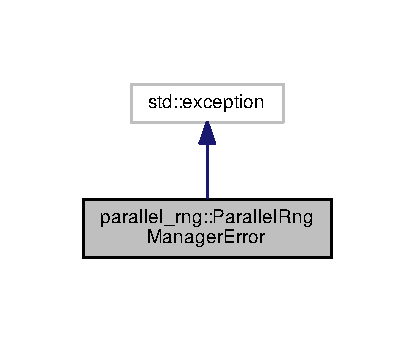
\includegraphics[width=198pt]{classparallel__rng_1_1ParallelRngManagerError__inherit__graph}
\end{center}
\end{figure}


Collaboration diagram for parallel\-\_\-rng\-:\-:Parallel\-Rng\-Manager\-Error\-:
\nopagebreak
\begin{figure}[H]
\begin{center}
\leavevmode
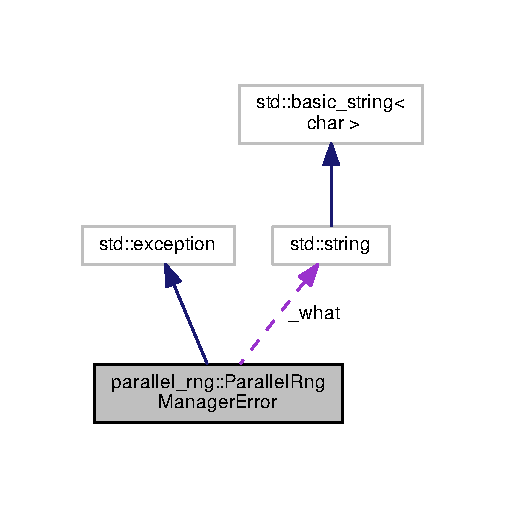
\includegraphics[width=243pt]{classparallel__rng_1_1ParallelRngManagerError__coll__graph}
\end{center}
\end{figure}
\subsubsection*{Public Member Functions}
\begin{DoxyCompactItemize}
\item 
\hyperlink{classparallel__rng_1_1ParallelRngManagerError_a4b2a32272aec6138e01b0ec2e78af926}{Parallel\-Rng\-Manager\-Error} (std\-::string \hyperlink{classparallel__rng_1_1ParallelRngManagerError_ac28661494c75c14d38cad8fdaccc9a63}{what})
\item 
const char $\ast$ \hyperlink{classparallel__rng_1_1ParallelRngManagerError_ac28661494c75c14d38cad8fdaccc9a63}{what} () const noexceptoverride
\end{DoxyCompactItemize}
\subsubsection*{Protected Attributes}
\begin{DoxyCompactItemize}
\item 
std\-::string \hyperlink{classparallel__rng_1_1ParallelRngManagerError_a446e23822c79bd7b8ce0dc2b4568d297}{\-\_\-what}
\end{DoxyCompactItemize}


\subsubsection{Detailed Description}


Definition at line 60 of file Parallel\-Rng\-Manager.\-h.



\subsubsection{Constructor \& Destructor Documentation}
\hypertarget{classparallel__rng_1_1ParallelRngManagerError_a4b2a32272aec6138e01b0ec2e78af926}{\index{parallel\-\_\-rng\-::\-Parallel\-Rng\-Manager\-Error@{parallel\-\_\-rng\-::\-Parallel\-Rng\-Manager\-Error}!Parallel\-Rng\-Manager\-Error@{Parallel\-Rng\-Manager\-Error}}
\index{Parallel\-Rng\-Manager\-Error@{Parallel\-Rng\-Manager\-Error}!parallel_rng::ParallelRngManagerError@{parallel\-\_\-rng\-::\-Parallel\-Rng\-Manager\-Error}}
\paragraph[{Parallel\-Rng\-Manager\-Error}]{\setlength{\rightskip}{0pt plus 5cm}parallel\-\_\-rng\-::\-Parallel\-Rng\-Manager\-Error\-::\-Parallel\-Rng\-Manager\-Error (
\begin{DoxyParamCaption}
\item[{std\-::string}]{what}
\end{DoxyParamCaption}
)\hspace{0.3cm}{\ttfamily [inline]}}}\label{classparallel__rng_1_1ParallelRngManagerError_a4b2a32272aec6138e01b0ec2e78af926}


Definition at line 65 of file Parallel\-Rng\-Manager.\-h.



\subsubsection{Member Function Documentation}
\hypertarget{classparallel__rng_1_1ParallelRngManagerError_ac28661494c75c14d38cad8fdaccc9a63}{\index{parallel\-\_\-rng\-::\-Parallel\-Rng\-Manager\-Error@{parallel\-\_\-rng\-::\-Parallel\-Rng\-Manager\-Error}!what@{what}}
\index{what@{what}!parallel_rng::ParallelRngManagerError@{parallel\-\_\-rng\-::\-Parallel\-Rng\-Manager\-Error}}
\paragraph[{what}]{\setlength{\rightskip}{0pt plus 5cm}const char$\ast$ parallel\-\_\-rng\-::\-Parallel\-Rng\-Manager\-Error\-::what (
\begin{DoxyParamCaption}
{}
\end{DoxyParamCaption}
) const\hspace{0.3cm}{\ttfamily [inline]}, {\ttfamily [override]}, {\ttfamily [noexcept]}}}\label{classparallel__rng_1_1ParallelRngManagerError_ac28661494c75c14d38cad8fdaccc9a63}


Definition at line 66 of file Parallel\-Rng\-Manager.\-h.



References \-\_\-what.



\subsubsection{Member Data Documentation}
\hypertarget{classparallel__rng_1_1ParallelRngManagerError_a446e23822c79bd7b8ce0dc2b4568d297}{\index{parallel\-\_\-rng\-::\-Parallel\-Rng\-Manager\-Error@{parallel\-\_\-rng\-::\-Parallel\-Rng\-Manager\-Error}!\-\_\-what@{\-\_\-what}}
\index{\-\_\-what@{\-\_\-what}!parallel_rng::ParallelRngManagerError@{parallel\-\_\-rng\-::\-Parallel\-Rng\-Manager\-Error}}
\paragraph[{\-\_\-what}]{\setlength{\rightskip}{0pt plus 5cm}std\-::string parallel\-\_\-rng\-::\-Parallel\-Rng\-Manager\-Error\-::\-\_\-what\hspace{0.3cm}{\ttfamily [protected]}}}\label{classparallel__rng_1_1ParallelRngManagerError_a446e23822c79bd7b8ce0dc2b4568d297}


Definition at line 63 of file Parallel\-Rng\-Manager.\-h.



Referenced by what().



The documentation for this class was generated from the following file\-:\begin{DoxyCompactItemize}
\item 
\hyperlink{ParallelRngManager_8h}{Parallel\-Rng\-Manager.\-h}\end{DoxyCompactItemize}

\section{File Documentation}
\hypertarget{ParallelRngManager_8cpp}{\subsection{Parallel\-Rng\-Manager.\-cpp File Reference}
\label{ParallelRngManager_8cpp}\index{Parallel\-Rng\-Manager.\-cpp@{Parallel\-Rng\-Manager.\-cpp}}
}


Fast auto rng for parallel openmp code.  


{\ttfamily \#include $<$random$>$}\\*
{\ttfamily \#include $<$thread$>$}\\*
{\ttfamily \#include \char`\"{}omp.\-h\char`\"{}}\\*
{\ttfamily \#include \char`\"{}Parallel\-Rng\-Manager/\-Parallel\-Rng\-Manager.\-h\char`\"{}}\\*
Include dependency graph for Parallel\-Rng\-Manager.\-cpp\-:\nopagebreak
\begin{figure}[H]
\begin{center}
\leavevmode
\includegraphics[width=350pt]{ParallelRngManager_8cpp__incl}
\end{center}
\end{figure}
\subsubsection*{Namespaces}
\begin{DoxyCompactItemize}
\item 
\hyperlink{namespaceparallel__rng}{parallel\-\_\-rng}
\end{DoxyCompactItemize}
\subsubsection*{Functions}
\begin{DoxyCompactItemize}
\item 
Seed\-T \hyperlink{namespaceparallel__rng_ae9d03797791785f0b9512fc2ef69bfb7}{parallel\-\_\-rng\-::generate\-\_\-seed} ()
\item 
Idx\-T \hyperlink{namespaceparallel__rng_a6165820e910d529d0287c1b1314be94e}{parallel\-\_\-rng\-::openmp\-\_\-estimate\-\_\-max\-\_\-threads} ()
\begin{DoxyCompactList}\small\item\em Use openmp to estimate the maximum number of threads that will be generated. \end{DoxyCompactList}\end{DoxyCompactItemize}


\subsubsection{Detailed Description}
Fast auto rng for parallel openmp code. \begin{DoxyAuthor}{Author}
Mark J. Olah (mjo@cs.\-unm D\-O\-T edu) 
\end{DoxyAuthor}
\begin{DoxyDate}{Date}
2016-\/2017 
\end{DoxyDate}


Definition in file \hyperlink{ParallelRngManager_8cpp_source}{Parallel\-Rng\-Manager.\-cpp}.


\hypertarget{ParallelRngManager_8h}{}\subsection{Parallel\+Rng\+Manager.\+h File Reference}
\label{ParallelRngManager_8h}\index{Parallel\+Rng\+Manager.\+h@{Parallel\+Rng\+Manager.\+h}}


Adapts T\+R\+NG parallel R\+NG to armadillo, maintaining a per-\/thread R\+NG.  


{\ttfamily \#include $<$cstdint$>$}\\*
{\ttfamily \#include $<$exception$>$}\\*
{\ttfamily \#include $<$functional$>$}\\*
{\ttfamily \#include $<$omp.\+h$>$}\\*
{\ttfamily \#include $<$armadillo$>$}\\*
{\ttfamily \#include $<$trng/lcg64\+\_\+shift.\+hpp$>$}\\*
{\ttfamily \#include \char`\"{}Parallel\+Rng\+Manager/\+Any\+Rng/\+Any\+Rng.\+h\char`\"{}}\\*
{\ttfamily \#include \char`\"{}Parallel\+Rng\+Manager/\+Aligned\+Array/\+A\+Array.\+h\char`\"{}}\\*
Include dependency graph for Parallel\+Rng\+Manager.\+h\+:\nopagebreak
\begin{figure}[H]
\begin{center}
\leavevmode
\includegraphics[width=350pt]{ParallelRngManager_8h__incl}
\end{center}
\end{figure}
This graph shows which files directly or indirectly include this file\+:\nopagebreak
\begin{figure}[H]
\begin{center}
\leavevmode
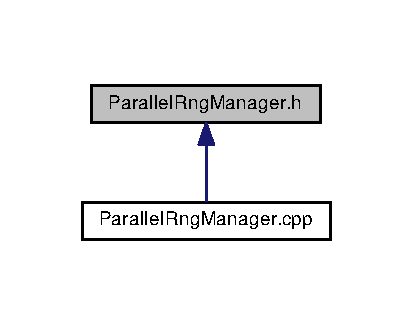
\includegraphics[width=199pt]{ParallelRngManager_8h__dep__incl}
\end{center}
\end{figure}
\subsubsection*{Classes}
\begin{DoxyCompactItemize}
\item 
class \hyperlink{classparallel__rng_1_1ParallelRngManagerError}{parallel\+\_\+rng\+::\+Parallel\+Rng\+Manager\+Error}
\item 
class \hyperlink{classparallel__rng_1_1ParallelRngManager}{parallel\+\_\+rng\+::\+Parallel\+Rng\+Manager$<$ Rng\+T, Float\+T $>$}
\end{DoxyCompactItemize}
\subsubsection*{Namespaces}
\begin{DoxyCompactItemize}
\item 
 \hyperlink{namespaceparallel__rng}{parallel\+\_\+rng}
\end{DoxyCompactItemize}
\subsubsection*{Macros}
\begin{DoxyCompactItemize}
\item 
\#define \hyperlink{ParallelRngManager_8h_a49b0c4ba8ba6a8ffa89bb4c8b91a38f1}{D\+E\+B\+U\+G\+\_\+\+A\+S\+S\+E\+RT}(...)
\item 
\#define \hyperlink{ParallelRngManager_8h_a2bbb5284a55381bafe1d369968b273e2}{A\+S\+S\+E\+R\+T\+\_\+\+S\+E\+T\+UP}(...)
\end{DoxyCompactItemize}
\subsubsection*{Typedefs}
\begin{DoxyCompactItemize}
\item 
using \hyperlink{namespaceparallel__rng_a4cb66b089d51a2a89cf6deac41c9b15f}{parallel\+\_\+rng\+::\+Default\+Parallel\+RngT} = trng\+::lcg64\+\_\+shift
\begin{DoxyCompactList}\small\item\em Suggested default Parallel\+R\+NG type. \end{DoxyCompactList}\item 
using \hyperlink{namespaceparallel__rng_a462b8721a1aabe3b86582e864640c707}{parallel\+\_\+rng\+::\+SeedT} = uint64\+\_\+t
\begin{DoxyCompactList}\small\item\em Use the true random interface to generate a truly random seed. \end{DoxyCompactList}\item 
using \hyperlink{namespaceparallel__rng_aa22fa3e339aee5927780aac099dfc6f3}{parallel\+\_\+rng\+::\+IdxT} = arma\+::uword
\end{DoxyCompactItemize}
\subsubsection*{Functions}
\begin{DoxyCompactItemize}
\item 
SeedT \hyperlink{namespaceparallel__rng_ae9d03797791785f0b9512fc2ef69bfb7}{parallel\+\_\+rng\+::generate\+\_\+seed} ()
\item 
IdxT \hyperlink{namespaceparallel__rng_a6165820e910d529d0287c1b1314be94e}{parallel\+\_\+rng\+::openmp\+\_\+estimate\+\_\+max\+\_\+threads} ()
\begin{DoxyCompactList}\small\item\em Use openmp to estimate the maximum number of threads that will be generated. \end{DoxyCompactList}\item 
{\footnotesize template$<$class RngT  = Default\+Parallel\+RngT, class FloatT  = double$>$ }\\Parallel\+Rng\+Manager$<$ RngT, FloatT $>$ \hyperlink{namespaceparallel__rng_a1442f14113d25568626a66f85c40e4ee}{parallel\+\_\+rng\+::make\+\_\+parallel\+\_\+rng\+\_\+manager} ()
\item 
{\footnotesize template$<$class RngT  = Default\+Parallel\+RngT, class FloatT  = double$>$ }\\Parallel\+Rng\+Manager$<$ RngT, FloatT $>$ \hyperlink{namespaceparallel__rng_a3d16c2aa5295d7ebeacbb87cb38c8e85}{parallel\+\_\+rng\+::make\+\_\+parallel\+\_\+rng\+\_\+manager} (SeedT seed)
\end{DoxyCompactItemize}


\subsubsection{Detailed Description}
Adapts T\+R\+NG parallel R\+NG to armadillo, maintaining a per-\/thread R\+NG. 

\begin{DoxyAuthor}{Author}
Mark J. Olah (mjo@cs.\+unm D\+OT edu) 
\end{DoxyAuthor}
\begin{DoxyDate}{Date}
2016-\/2017 
\end{DoxyDate}


\subsubsection{Macro Definition Documentation}
\index{Parallel\+Rng\+Manager.\+h@{Parallel\+Rng\+Manager.\+h}!A\+S\+S\+E\+R\+T\+\_\+\+S\+E\+T\+UP@{A\+S\+S\+E\+R\+T\+\_\+\+S\+E\+T\+UP}}
\index{A\+S\+S\+E\+R\+T\+\_\+\+S\+E\+T\+UP@{A\+S\+S\+E\+R\+T\+\_\+\+S\+E\+T\+UP}!Parallel\+Rng\+Manager.\+h@{Parallel\+Rng\+Manager.\+h}}
\paragraph[{\texorpdfstring{A\+S\+S\+E\+R\+T\+\_\+\+S\+E\+T\+UP}{ASSERT_SETUP}}]{\setlength{\rightskip}{0pt plus 5cm}\#define A\+S\+S\+E\+R\+T\+\_\+\+S\+E\+T\+UP(
\begin{DoxyParamCaption}
\item[{}]{...}
\end{DoxyParamCaption}
)}\hypertarget{ParallelRngManager_8h_a2bbb5284a55381bafe1d369968b273e2}{}\label{ParallelRngManager_8h_a2bbb5284a55381bafe1d369968b273e2}


Definition at line 45 of file Parallel\+Rng\+Manager.\+h.

\index{Parallel\+Rng\+Manager.\+h@{Parallel\+Rng\+Manager.\+h}!D\+E\+B\+U\+G\+\_\+\+A\+S\+S\+E\+RT@{D\+E\+B\+U\+G\+\_\+\+A\+S\+S\+E\+RT}}
\index{D\+E\+B\+U\+G\+\_\+\+A\+S\+S\+E\+RT@{D\+E\+B\+U\+G\+\_\+\+A\+S\+S\+E\+RT}!Parallel\+Rng\+Manager.\+h@{Parallel\+Rng\+Manager.\+h}}
\paragraph[{\texorpdfstring{D\+E\+B\+U\+G\+\_\+\+A\+S\+S\+E\+RT}{DEBUG_ASSERT}}]{\setlength{\rightskip}{0pt plus 5cm}\#define D\+E\+B\+U\+G\+\_\+\+A\+S\+S\+E\+RT(
\begin{DoxyParamCaption}
\item[{}]{...}
\end{DoxyParamCaption}
)}\hypertarget{ParallelRngManager_8h_a49b0c4ba8ba6a8ffa89bb4c8b91a38f1}{}\label{ParallelRngManager_8h_a49b0c4ba8ba6a8ffa89bb4c8b91a38f1}


Definition at line 40 of file Parallel\+Rng\+Manager.\+h.


\hypertarget{README_8md}{}\subsection{R\+E\+A\+D\+M\+E.\+md File Reference}
\label{README_8md}\index{R\+E\+A\+D\+M\+E.\+md@{R\+E\+A\+D\+M\+E.\+md}}

%--- End generated contents ---

% Index
\newpage
\phantomsection
\addcontentsline{toc}{section}{Index}
\printindex

\end{document}
